\section[Introduction]{Introduction}
\begin{frame}{Historique}
    \begin{figure}
        \centering
        \subfigure[Logo \LaTeX]{
\includegraphics[height=1.5cm]{LaTeX_logo.png}} \hfill
        \subfigure[Leslie Lamport]{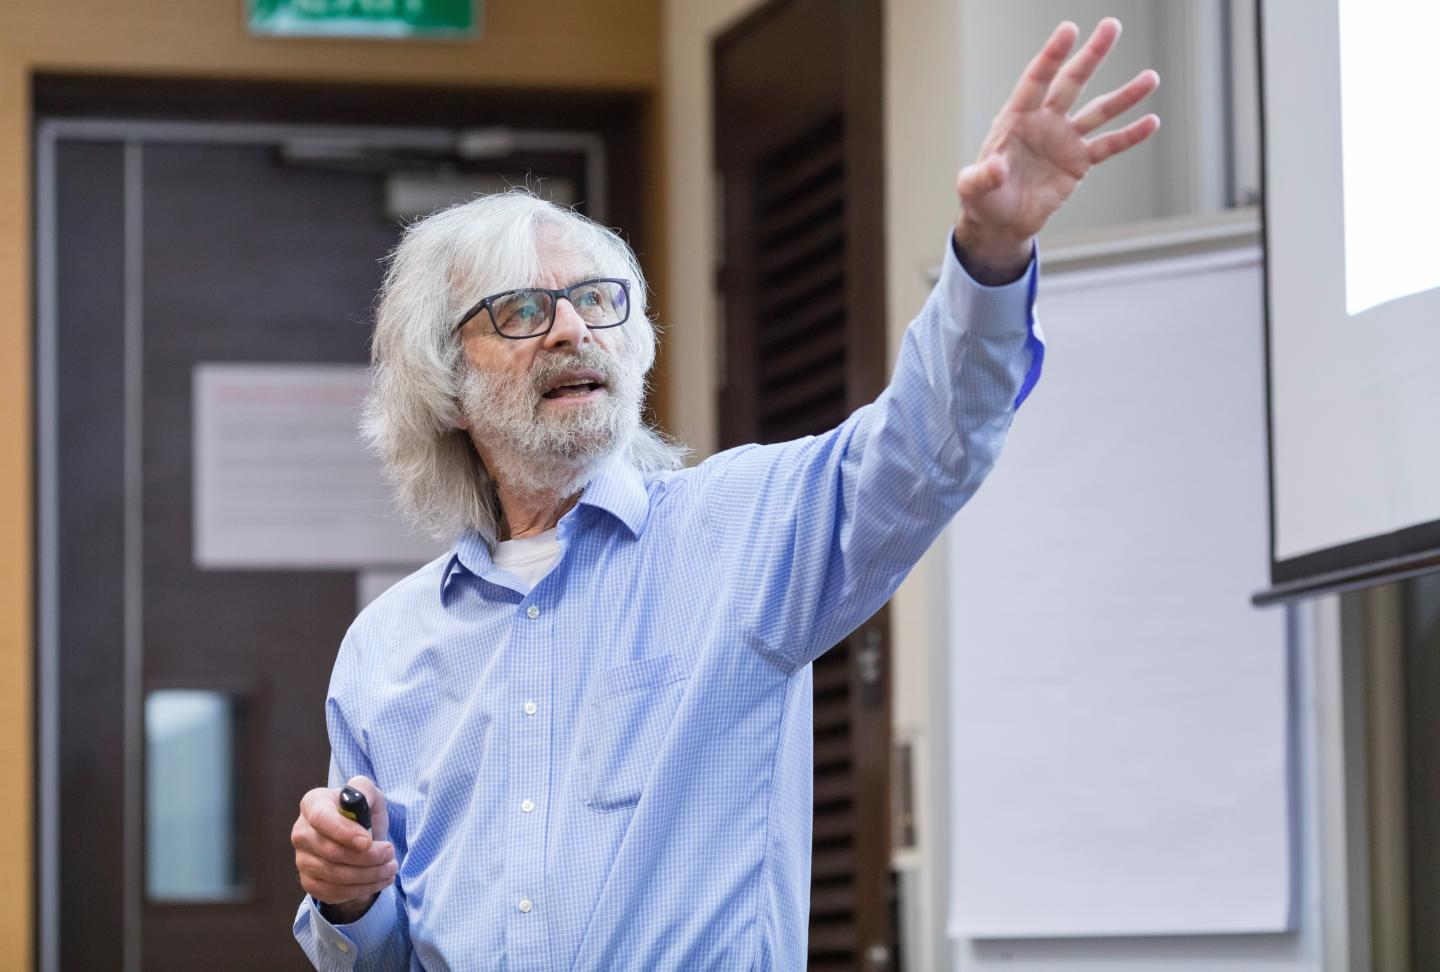
\includegraphics[width=5cm]{Leslie_Lamport2.jpg}}
    \end{figure}
    
    \begin{itemize}[label=$\triangleright$]
        \item Prononciation \og Lah-tech \fg{} 
        \item Langage et système de composition de document
        \item Créé par Leslie Lamport, début des années 1980
        \item Utilisé principalement dans les domaines académiques mais aussi techniques
    \end{itemize}
\end{frame}

\begin{frame}{Principe d'utilisation}
    \begin{itemize}[label=$\triangleright$]
        \item Langage informatique de balisage
        \item Editeur de texte (NotePad++ et non MS Word)
        \item Macro-commandes et compilateur
    \end{itemize}
\end{frame}

\begin{frame}{Installation}
    \begin{itemize}[label=$\triangleright$]
        \item Editeur et compilateur online : \href{https://fr.overleaf.com}{https://fr.overleaf.com}
        \item MikTeX et TexMaker
        \item TexLive et VisualStudioCode
    \end{itemize}
\end{frame}

\begin{frame}{Installation -- Overleaf}
    \begin{exampleblock}{Avantage}
        \begin{itemize}[label=$\triangleright$]
            \item Tous les packages installés
            \item Disponible partout (online)
            \item Moins de problèmes de compilation
            \item Banque de templates variées
        \end{itemize}
    \end{exampleblock}
    \bigskip
    $\Longrightarrow$ Il suffit de faire simplement un compte étudiant (0.-/mois). \\
    $\Longrightarrow$ Possibité de faire des documents partagés entre plusieurs membre en créant un compte avec une seule adresse mail commune à tous.tes les collaborateur.rices.
\end{frame}

\begin{frame}{Installation -- TexMaker}
    \begin{enumerate}
        \item \underline{Installation de \texttt{MikTex} :} \internet{https://miktex.org/download} \\
        C'est l'environnement de développement pour produire des fichiers pdf à partir de fichier \texttt{.tex}
        \item \underline{Installation de TexMaker :} \internet{https://www.xm1math.net/texmaker/download_fr.html} \\
        C'est un logiciel tourné vers les débutants avec un maximum d'aide et de raccourci. Il permet de créer et d'écrire les fichiers \texttt{.tex} ainsi que de les compiler.
    \end{enumerate}
\end{frame}

\begin{frame}{Installation -- VisualStudioCode}
    \begin{enumerate}
        \item \underline{Installation de TeX Live :} \internet{http://mirror.ctan.org/systems/texlive/tlnet/install-tl-windows.exe} \\
        Environnement de développement pour produire des fichiers pdf à partir de fichier \texttt{.tex}
        \item \underline{Installation de Visual Studio Code :} \internet{https://www.xm1math.net/texmaker/download_fr.html} \\
        Logiciel pour éditer les fichiers \texttt{.tex}.
        \item \underline{Installation de l'extension LaTeX Workshop :} permet de compiler et créer le fichier \texttt{.pdf}
    \end{enumerate}
    \begin{exampleblock}{Conseil}
        VS Code permet de paramétrer son environnement comme on le souhaite.
        Il peut aussi être couplé avec Git (\& GitHub).
        N'hésitez pas à regarder des tutos vidéos.
    \end{exampleblock}
\end{frame}